\section{Краткие теоретические сведения}

Что такое <<открытая система>>?

Открытой может быть названа любая система (компьютер, вычислительная сеть, ОС, программный пакет, другие аппаратные и программные продукты), которая построена в соответствии с открытыми спецификациями.

Под открытыми спецификациями понимаются опубликованные, общедоступные спецификации, соответствующие стандартам и принятые в результате достижения согласия после всестороннего обсуждения всеми заинтересованными сторонами.

Использование при разработке систем открытых спецификаций позволяет третьим сторонам разрабатывать для этих систем различные аппаратные или программные средства расширения и модификации, а также создавать программно-аппаратные комплексы из продуктов разных производителей.

Модель ВОС (взаимодействия открытых систем) - это концептуальная модель процесса коммуникаций, основанная на разбиении этого процесса на несколько функциональных уровней, каждый из которых взаимодействует только со своими непосредственными соседями, аналогично тому, как это происходит при разработке операционных систем. 

\begin{figure}[H]
    \centering
    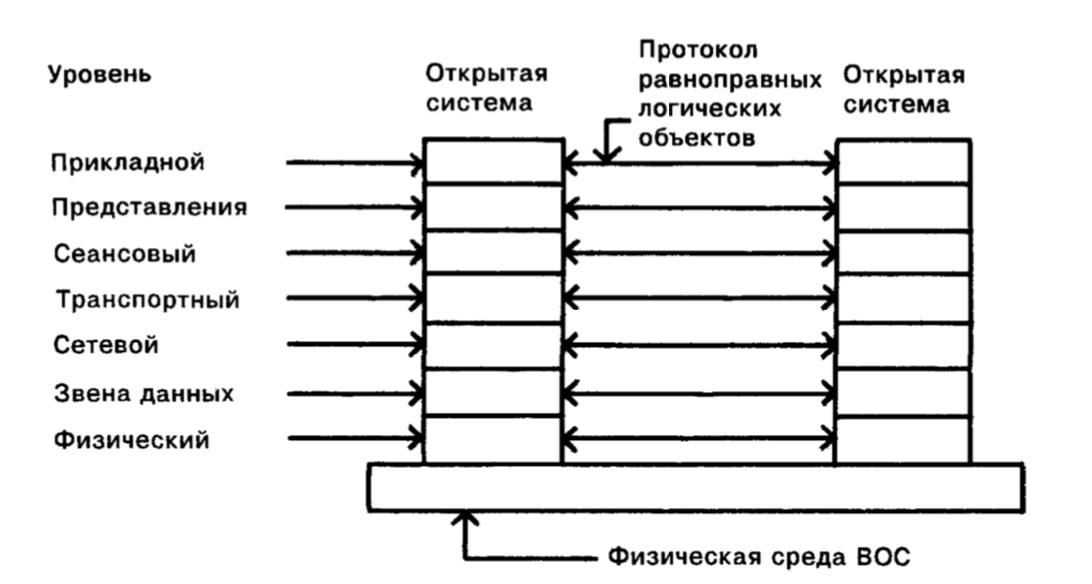
\includegraphics[width=.9\textwidth]{img/vos.png}
    \caption{эталонная модель взаимосвязи открытых систем}
\end{figure}


Эталонная модель интероперабельности представляет собой развитие семиуровневой базовой эталонной модели взаимосвязи открытых систем согласно ГОСТ Р ИСО/МЭК 7498-1-99)

\begin{figure}[H]
    \centering
    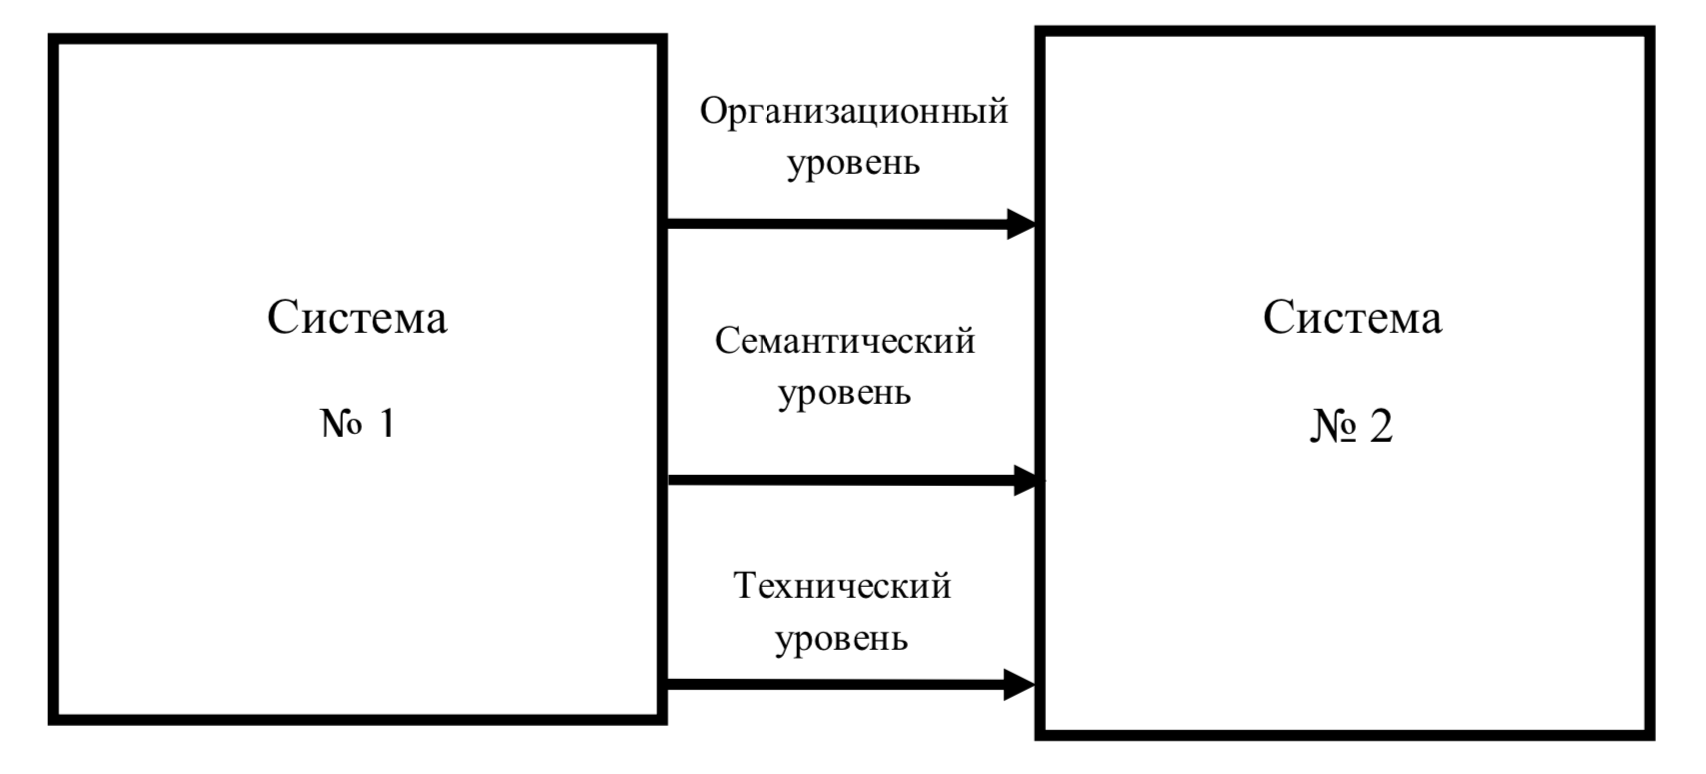
\includegraphics[width=.9\textwidth]{img/intero.png}
    \caption{эталонная модель интероперабельности}
\end{figure}



Технический уровнеь описывает синтаксис или форматы передаваемой информации, заостряя внимание на том, как представлена информация в коммуникационной среде. Технический уровень включает такие ключевые аспекты, как открытые интерфейсы, службы связи, интеграция данных и промежуточный слой программного обеспечения (Middleware), представление и обмен данными, службы доступности и защиты информации. Техническая интероперабельность достигается, главным образом, за счет использования стандартных протоколов связи типа TCP/IP.

Семантический уровень описывает семантические аспекты взаимодействия, т. е., содержательную сторону обмениваемой информации. Семантическая интероперабельность позволяет системам комбинировать полученную информацию с другими информационными ресурсами и обрабатывать ее смыслового содержания. Семантическая интероперабельность достигается за счет применения стандартов типа XML.

Организационный уровень акцентирует внимание на прагматических аспектах взаимодействия (деловых или политических). На этом уровне согласуются бизнес-цели, и достигаются соглашения о сотрудничестве между административными органами, которые хотят обмениваться информацией, хотя имеют отличающиеся внутреннюю структуру и процессы. Более того, организационная интероперабельность имеет свой целью удовлетворить требования сообщества пользователей: службы должны стать доступными, легко идентифицироваться и быть ориентированными на пользователя. Организационная интероперабельность достигается не за счет применения стандартов (нормативно-технических документов), а за счет применения нормативно-правовых документов (соглашений, конвенций, договоров о сотрудничестве).

